\chapter{Background}
\label{c:Background}

\section{Program Comprehension}

\section{Static vs. Dynamic Analysis}

\section{Modeling of Objects, States, and Interactions}
\label{s:BackgroundModeling}

\subsection{Object Diagrams}
\label{ss:BackgroundModelingObject}

\begin{figure}
	\centering
	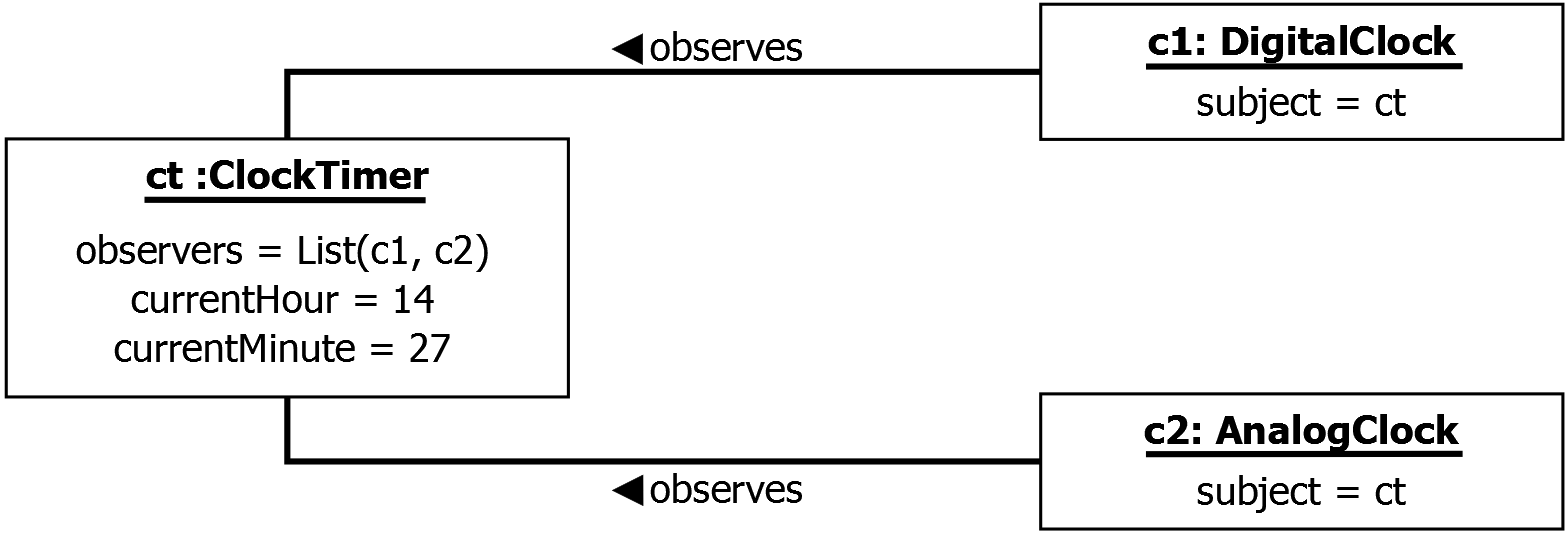
\includegraphics[width=0.7\textwidth]{../images/02-Object}
	\caption[TOC Caption]{UML Object Diagram}
	\label{fig:ModelingObject}
\end{figure}

Object diagrams \cite{rumbaugh_unified_2010} are structural diagrams that can be seen as concretization of a class diagram for a definite point in time.
As such, their notation (cf. Figure \ref{fig:ModelingObject}) covers instances and their state as well as links between instances.
The description of an instance includes an optional identifier, the type of the instance, and a list of attributes and their values.
Links can be annotated with roles and link names, whereby the latter are equipped with indicators for the reading direction.
In addition, links can be declared as forward-navigable and non-backward navigable.

Object diagrams allow the diagram creator to place objects freely on the two-dimensional canvas.
This has the advantage that objects that are closely related can be depicted in spatial proximity.
Likewise, groups of objects that are not related can be placed in different parts of the canvas.
Thus, a map of the system's runtime structure can be created that allows the observer to intuitively get an understanding of the parts of a system and their connections.

\subsection{Sequence Diagrams}
\label{ss:BackgroundModelingSequence}

\begin{figure}
	\centering
	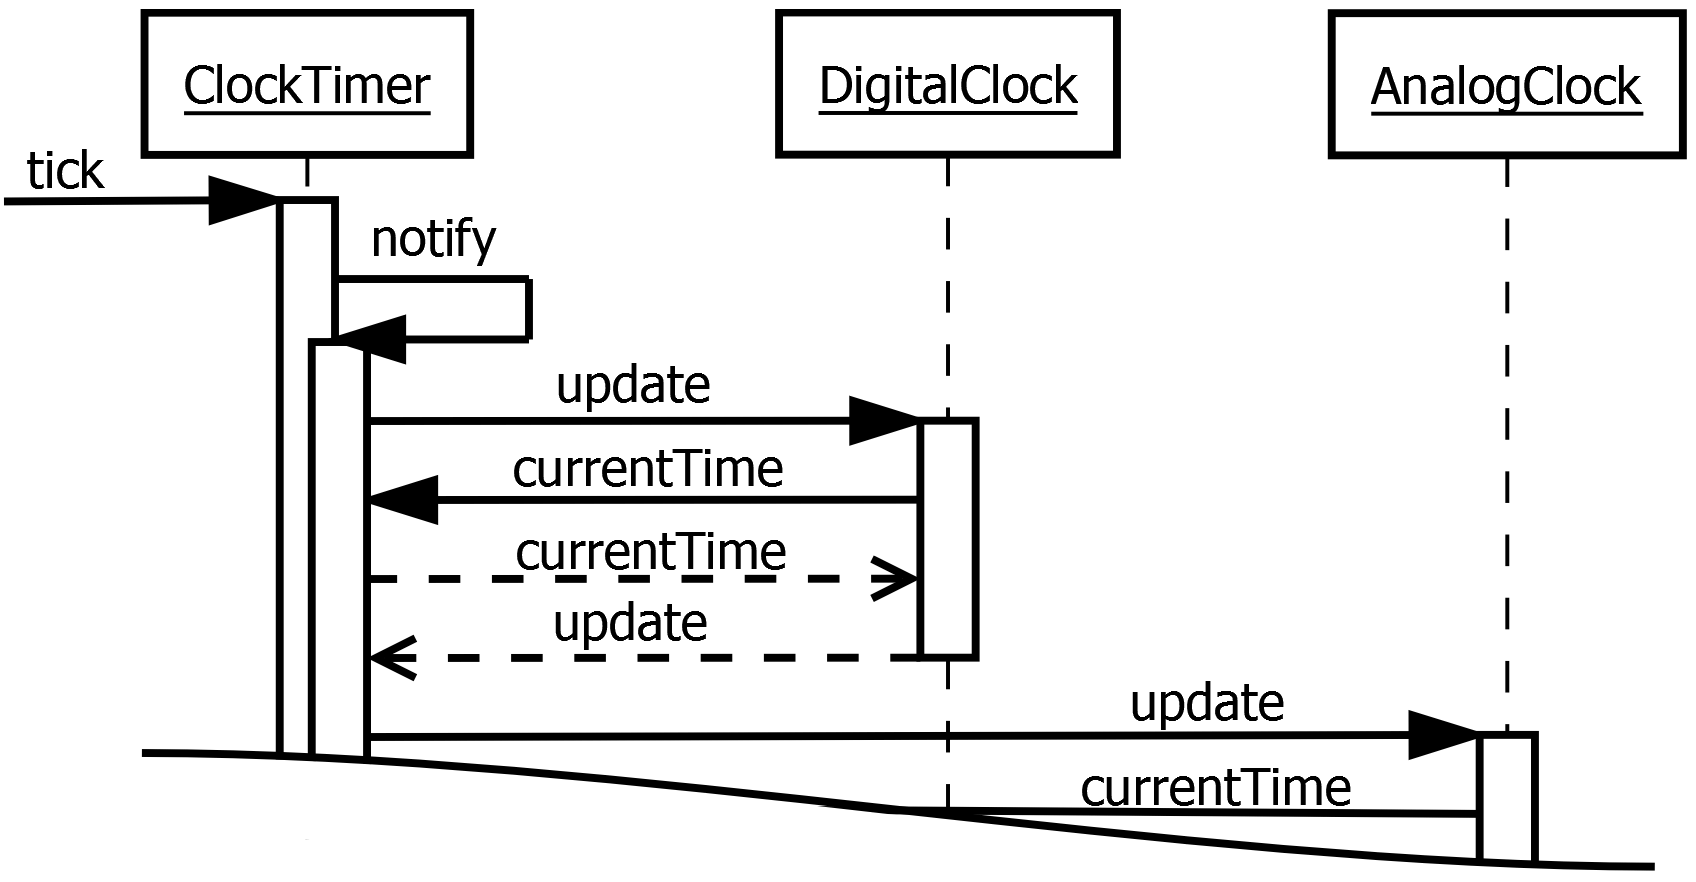
\includegraphics[width=0.6\textwidth]{../images/02-Sequence}
	\caption[TOC Caption]{UML Sequence Diagram}
	\label{fig:ModelingSequence}
\end{figure}

Sequence diagrams \cite{rumbaugh_unified_2010} are used to model the interaction of objects.
Thereby, the focus is on the exchange of messages in a specific scenario rather than the depiction of all possible execution branches.
The fundamental notation elements are depicted in Figure \ref{fig:ModelingSequence}.

Objects and their lifelines are aligned along the horizontal axis.
Execution specifications on the lifelines indicate whether an object is currently participating in a computation.
Messages between two objects are represented by arrows.
They are aligned along the vertical axis according to their chronological appearance.
Each message is complemented by a return message which indicates the end of a method invocation and which is depicted as dashed arrow.
Apart from those basic components, sequence diagrams also can be used to model duration constraints, state invariants and asynchronous behavior.
However, those advanced notation elements are of no great importance in our context.

Sequence diagrams have two major advantages.
Firstly, they feature an inherent chronological ordering, which makes following the communication thread easier for the observer.
Secondly, the automatic generation of sequence diagrams from execution traces is comparatively trivial and consequently fast, as no computation-intensive layout strategies have to be performed.
One could argue that the arrangement of the objects on the horizontal axis should be adjusted to minimize the distance between objects that exchange messages.
This optimization would certainly introduce computational complexity, but does not seem to be a common practice among the wide range of tools offering the generation of sequence diagrams that are reviewed in the related work section (cf. Chapter \ref{c:relatedwork}).

\subsection{Communication Diagrams}
\label{ss:BackgroundModelingCommunication}

\begin{figure}
	\centering
	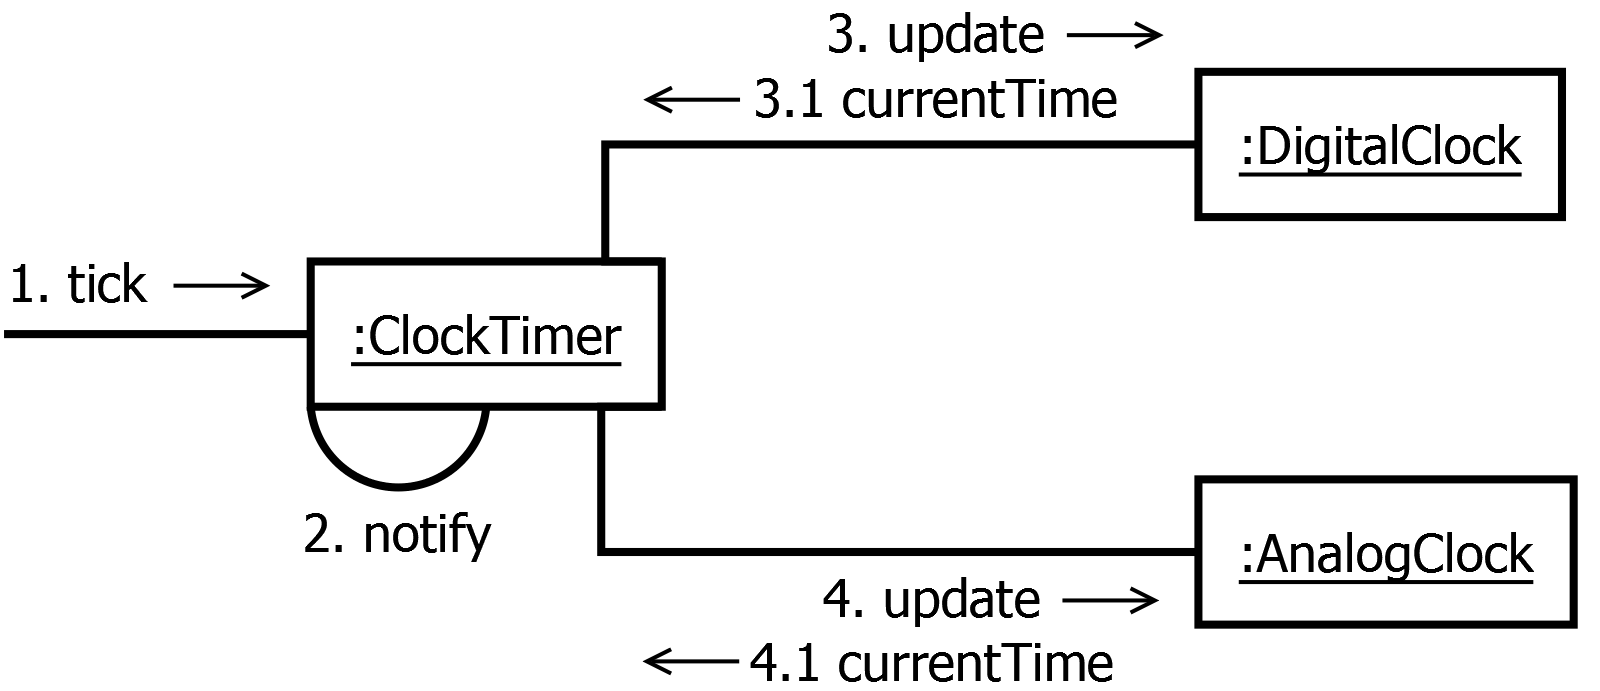
\includegraphics[width=0.6\textwidth]{../images/02-Communication}
	\caption[TOC Caption]{UML Communication Diagram}
	\label{fig:ModelingCommunication}
\end{figure}

\subsection{Discussion}
Due to the fact that the Unified Modeling Language makes a strict distinction between structural and behavioral diagrams, none of them offers a combined view on object interactions as well as the internal state of objects.
However, to understand the behavior of object-oriented systems, it is important to get an insight into both.
Interactions have to be depicted in order to make the behavior of a system perceivable to the observer.
To understand why a systems behaves the way it does, the internal state of objects has to be unveiled.

Apart from this fundamental problem, the diagrams all have drawbacks of their own that make them inadequate for our objectives.

\section{Challenges}